Hash tables generalise the simple notion of direct addressing making effective uise of the ability to examine an arbtrary element of an array in $O(1)$ which we know is not affordable when the key universe is big, because it requires space which is proportional to the size of the universe. 
\subsection{Direct Addressing Table}
Suppose for instance that an application needs a synamic set in which each elemtn has a keu drqwn from the universe $U 0 \{0,1,\ldots m-1\} $ where $m$ is not too large and no towo element share the same key (indiex of the direct addressing table).
A direct addressing table is a indexable structure of size $m$ where each key of the universe has a one to one correspondence to one slot of the table. 
Dictionary operations can be performed as follows:

\begin{algorithm}
\Fn{SEARCH (T,k)}{
	$return T[k]$
 }
 \Fn{INSERT (T,x)}{
	$T[tokey(x)] = x$
 }
 \Fn{DELETE (T,x)}{
	$T[tokey(x)] = NIL$
 }
\caption{DIRECT ADDRESSING OPERATIONS}
\end{algorithm}

	\begin{figure}
	\label{fig:directaddressing}
	\centering
		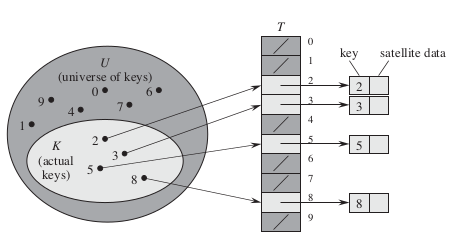
\includegraphics{direct_addressing}
	\end{figure}

where $tokey$ is a function which takes an object $x$ and maps it to an integer in the interval $0\ldots m-1$. Such function is called $hashing function$. 
%---Problem------------
\begin{problem}
\textit{Suppose that a dynamic set S is represented by a direct-address table $T$ of length $m$. Describe a procedure that finds the maximum element of $S$. What is the worst-case performance of your procedure?}.

\begin{solution}
The direct addressing table is not sorted so binary search cannot be used. Only option is a linear scan.
\end{solution}
\end{problem}

Hash tables use addressing with indices as basic idea, but overcome the problem of using large space by using space which is proportional to the number of keys actually stored. The main idea is that we can compute an index from each key to be inserted, in $O(1)$ and use that index as the index of the array location where to store the object. Obviously a because the number of slots is less than the number of possible keys it is possible for two key to be stored at the same location hyelding to a \textit{collision}. There are various effective approach to handle collision which will be describer in the following sections.
In a hash table an element with is stored at slot $h(x)$ where $h$ is an hash function which maps the universe of keys $U$ into slots of the hash table.
\[
h(x): U \mapsto \{0,1,\ldots,m-1\}
\]
with $m$ typically much smaller than $|U|$. The hitch is that (pigeone priciple) two object may be assigned the same slot (they hash to the same slot). This situation is called a \textbf{collision}. There are several tecnquiques to deal with collisions such as 
\begin{enumerate}
\item chaining
\item open addressing
\item linear probing
\item quadratic probing
\item random probing
\end{enumerate}
Of course the best scenario is to avoid collision altogether but since the size of the universe if bigger than the size of the hash table there always exists at least a couple of object which will hash to the same slot. The hash function should, in order to minimize collision as much random as possible (remaining deterministic obviously). The word hash means to mix and it somehow evoke what this function does. It mixes data taken from the object in order to provide a random looking index to be used as an index of the hash table.

\subsection{Collision resolution by chaining}
In chaining, all the elements that hash to the same slot are placed into the same linked-list. The hash table can be viewed, infact, as an array of linked list where each node of the list contains apointer to the object stored.
Dictionary operation can so be performed in average case $O(1)$ as follows:
\begin{algorithm}
\Fn{SEARCH (T,x)}{
	$LIST-SEARCH(T[h(x)]$ 
	\tcc{Worst case - O(n) we will see that average case is much better O(1)}
 }
 \Fn{INSERT (T,x)}{
	$LIST-INSERT-HEAD(T[h(x)],x)$
	\tcc{O(1)}
 }
 \Fn{DELETE (T,x)}{
	$LIST-DELETE(T[h(x)],x)$
	\tcc{O(1) is list are doyhbly linked or O(n) if singly linked}
 }
\caption{Hash table - chaining dictionary operations }
\end{algorithm}

\subsubsection{ANALYSING PERFORMANCE OF HASHING WITH CHAINING}
Given an hash table $T$ we define the \textbf{load factor} ad the ration $\alpha=\frac{n}{m}$ where $n$ is the actual number of element stored into the hash table and $m$ is the dsize of the table.
The worst case scenario for hashtable with chaining is very bad. When all the inserted element hash to the same slot the seach procedure degrade to linear search in a list, with complexity $\Theta(n)$. We will show now that hash table performs much better on the average case and when certain operation such as enlarging or shrinking are performed carefully.
The main question here is: what is the complesxity for a hash table lookup operation? We evaulate the complexity of this operation with the length of the list being searched. A lookup operation may be succesful or unsuccesful. Analysing the former case is easy, since assuming that object are hashed with a \textbf{simple uniform hash function}\footnote{A function that hashes each object to one of the slots with uniform probability $Pr(h(obj)=j)=\frac{1}{m}$ and independently of the already hashed objects} while the latter requires a bit more work. Infact if we denote the length of the list $T[k]$  at location $k$ as $n_k$ then $n=\sum_{i=1}^{m-1} n_i$. The expected value for $n_j$ is then $\alpha$. 

In a unsuccesful lookup operation the list $T[j]$ must be traversed completly from head to tail giving so a complexity of $\Theta(1+\alpha)$ (computing of $j$ via the hasing function, plus the length of the list being searched). 
In a succesful lookup operation the list being search will be searched half way through on average case so the complexity will be $\approx\Theta(1+\frac{\alpha}{2})$.
Another approach would be to consider that supposing that the element being search lie in at location $j$ of list $T[l]$ all the element at indices $j-1,j-2,\ldots,0$ are inserted \textbf{after} the element being searched (because the insert operation push the element at the head of the list. In a succesful search then we examine all the element that have been inserted before. What is the probability that two element hash to the same slot? Again, $\frac{1}{m}$ because of the simple uniform hashing assumpion. So the cost of a single lookup is $1$ plus the number of element inserted after $j$ that hash to the same location of element $j$: 
\[
1+ \sum_{j=i+1}^n = \frac{1}{m}  = 1 + \frac{1}{m} \sum_{j=i+1}^n 1 =  1 + \frac{1}{m} (n-j)
\]
Taking the average over $n$ insertion we have 
\[
\frac{1}{n} \sum_{i=1}^n (1 + \frac{1}{m} (n-j)) = \frac{1}{n}(n + \frac{1}{m} \sum_{i=1}^n n -  \sum_{i=1}^n i)  = 1 +\frac{1}{nm} (n^2 -  \frac{n(n+1)}{2} ) = 1 + \frac{n^2}{nm} - (\frac{n^2}{2} + \frac{n}{nm}) = 1+ \alpha - \frac{\alpha}{2} + \frac{1}{2m}
\]
which is $\Theta(1+\alpha)$

What does this mean? That if we can keep  the value of $\alpha$ \textbf{constant} then we can perform all the dictionary operation in $O(1)$ average case! How can we keep $\alpha$ constant? If we keep $m$ is of the same order of $n$ then we have $\alpha = O(m)/n =(1)$ This tells us that the size of the hash table should be of the same order of the number of element stored in the has table itself. If we can ensure this invariant then dictionary operation can be performed in \textbf{constant time}!

\subsubsection{Alternative to Linked Lists}
Chaning with linked list in not obviouly the only possible solution. If we know that out universe is totally orderable than we could store the collisions in a binary search tree insted lowering the complexity from $\Theta(1+\alpha)$ to $\Theta(a+log(\alpha)$.


\subsection{Hash Functions}
A good hashing function satisfies the assumpion of simple uniform hashing. This condition is not easy to ensure a priori and is sometimes impossible to check because we rarly know the probability distribution of the key drwan. More importantly this keys may not be drawn independenlty. 
Heuristic are emplaced in the design of good hashing functions. For example in a compiler symbols table, it would be good for two similar words to hash in different slots (since for example two symbols like \texttt{pt} and \texttt{pts} may often occur in the same listing). 
Keys and object are often interpreted as natural numbers (and an important part of the hashing process is how we interpret the object as natural numbers. For instance a string may be interpreted as the sum of the ASCII values of all the character\footnote{Note that this is a terrible interpretation for a string since all the permutation of the same string willl produce the same key value!}). This key is then passed to another function which maps the keys into the most appropriate slot in the hash table. 

\subsubsection{Divison Method}
In the division method a key $k$ is mapped into one of the $m$ slots by taking the reminder of $k$ divided by $m$ (usually $ k> m$)
\[
h(m,k) = k \:mod\: m
\]
This methos is quite fast since it only requires a division. When using the divison method the size of the table, $m$ should not be a power of two since the division of $\frac{m=2^p}{k}$ consist of the p-lowest bits of $k$. For example let $m = 2^9 = 256_{10} = 010000000_2$ and $ k=300_{10}  = 100101010_2 \mapsto $ $k \: mod \:m = 000101010_2$ 
With this method the best choice is  prime number. But choosing $m$ prime does not solve all the problem or makes this method \textit{perfect} algtogether. All integer of the form $x+am$ will hash to the same slot $x$! Is quite easy then for a malicious agent to come up with a bad set of values that all hash to the same bucket.

\subsubsection{Multiplication Method}
The multiplication method operates in two steps: 
\begin{enumerate}
\item We multiply $k$ by a constant (called \textbf{salt}, chosen at creation time and remaining fixed for the entire lifetime of the hash table) $0<A<1$ and extract the fractional part of the result.
\item We then multiply this value by $m$ and take the floor of the result.
\end{enumerate}

\[
h(m,k) = \left \lfloor{m(Ak \: mod \: 1)}\right \rfloor 
\]
For instance suppose the key is $102$ and $A=\phi \approx 0.6180339887$ and $m = 30 $. The bucket is computed as follows:
\[
30 (\phi*102 - \left \lfloor \phi*102 \right \rfloor  ) =  \left \lfloor{30(63.0394668474 - 63 )}\right \rfloor = \left \lfloor{30*0.394668474}\right \rfloor  = \left \lfloor{11.84005422}\right \rfloor  = 11
\]
Since the fractional part of $Ak$ is a number always smaller than one, $h(m,k)$ is unsured to be in the interval $[0,m-1]$. A good advantage of this method is that the value of $m$ is not critical and infact we often choose $m$ to be a power of two since we can easily implement the method using shifts operators.


\begin{enumerate}
\item choose $m=2^p$
\item multiply $w$ bits of $k$ with $w$ bits of $(A *2^w)$ and we obtain a $2^w$ word number.
\item Extract the first $p$ bits of the lower hald of this product.
\end{enumerate}
A good choice as suggested by Knut is the  golden ration $\phi$.

Another good example in this class of hash function was analyzed by \textit{Dietzfelbinger et al.} in 1997, called binary multplicative hashing. The goal is to hash \textit{w}-bit integers (word size integer) to \textit{l}-bits (label) integers. 
we define such function as 
\[
d_a (x) = \left \lfloor{\frac{(ax) mod 2^w}{2^{w-l}}}\right \rfloor 
\]
with $a \in \{1,2,\ldots m-1\}$

\begin{lstlisting}[language=c++, caption="Multiplicative method hashing"]
typedef unsigned int uint;
#define INT_SIZE (32)
 int hash(const uint m,const  uint k, const uint a, const uint hash_size) {
 	return (a*k) >> (INT_SIZE-hash_size) 
 	//division by powers of 2 is equivalent to a right shift
 }

\end{lstlisting}
Note that the product $ak$ may be a $2^{2 \times INT\_SIZE}$ number, but this would cause overflow, so only the lower \texttt{INT\_SIZE} of the resulting product will be kept. Right shifting by the right amount will do the job of isolate the inner $l$ portion of the number. 
For instance consider the following listing:

\begin{lstlisting}[language=c++]
#include <iostream>
using namespace std;
typedef unsigned int uint;
int main() {
	uint a = 523456;
	uint res= a*a; //overflow
	cout<<(uint)res<<" "<<a<<endl;
	return 0;
}
\end{lstlisting}
\texttt{res} variable contains the number $3423244288$ which is the wrong answer since $523456^2=274006183936$. $3423244288$ correspond is a 32-bit integer which corresponds to the first 32-bits of the 64-bits number $274006183936$. $3423244288 = 274006183936 mod 2^{32}$.

\subsubsection{Universal Hashing}

Any possible scheme is vulnerable to the fact that is alway possible to choose $n$ objects whose keys maps to the same bucket, yelding as we know to the very bad $\Theta(n)$ lookup. The only approach that overcome this issue is for the hashing function to hash keys \textit{randomly} and \textit{indeentently}. In unversal hashing we select at the beginning of the the execution (at hash table  creation time if working in a object oriented programming environment) a suitable hash function from a set well designed class of functions. We will use randomizaion in the costruction of the hash function in ordder to ensure that for any sequence of element inserted in the table the expected performance will be good (i.e. the horrific $\Theta(n)$ lookup would occuper with a very little probability). This is the same kind of expectation quicksort assumes when choosing the pivot element.

\textit{To summarise when the keys to be inserted are uniformly drawn from a universe of keys is not difficould to come up with an hash function that distribute them uniformly across all the buckets meaning that the probability of collisions between any of two keys is the $\frac{1}{m}$ (any bucket at any time is equally likely to be chosen by the hash function). The main caveau is that the any assumption on the distribution of the keys to be inserted is not realistic manily because in real life keys are not drawn randomly, then because there could alway be the case then an adversary would attack our system submitting a patological sequence of keys which will hash to the same bucket. So a much more approach is to  make no asumption on the distribution of the keys and let randomess come into play in the definition of the hash function itself which is not now fixed. Looking now at the average running time of all the hash table operations withouth, again any assumpion on the distribution of the keys. An adversary cannot find a \textbf{bad sequence of keys} since the hash function is not known \textbf{a priori}. Randomess, which willl ensure good average case behaviour is in the definition of the hash function!} 

A family of function $\mathbb{H}$ is a  \textbf{universal hash function family} if each function the probability that two element collide is at most $\frac{1}{m}$ i.e. given two elements $x,y \in U$, $\forall h \in \mathbb{H}$ we have $Pr(h(x) = h(y)) \geq \frac{1}{m}$ (Sometimes this probability may be $O(\frac{1}{m})$ and the family is called $\epsilon$-almost universal). Not that universality does not implies uniformity\footnote{The propoerty such that all the possible hash values are equally likely to be returned. $Pr(h(x)=z) = \frac{1}{m}$}. Note also that uniformity is not terribly useful and is not a string enough condition to ensure good hash table performance on average. Take for instance the set $\mathbb{K} = \{ k_a(x) = a \: : 0\geq a<m\}$ of  constant function. This set is perfectly uniform in the sense that picking a random function $k_a$ at random each slot is equally likely to be choosen as destination slot. Probability that object $x$ hashes to slot $l$ is the probability that function $k_l$ is picked up at random from the set $\mathbb{K}$ which clearly is $\frac{1}{m}$. That is why minimizing the number of collision is much more important. The set $\mathbb{K}$ is uniform but is not unversal (according th the following definition) because the probability that picking up a random function $k_a$ and given two keys $x,y$ they hash to the same location is not less than $\frac{1}{m}$ but is $1$.


\begin{framed}
\textbf{Lineary of expectation} \hfill \\
By linearity of expectation we mean that the \textbf{expected value} of the sum of a random variable is equal to the sum of their individual expected values. It is essentially a weighted average of possible outcomes. Suppose we are interested in the expected value of the sum of $K$ dices. Calculating the the sum the usual way is tedious. We have to sum up all possible outcomes and divides by the total number of outcomes to get the expected values. 

\begin{tabular}{|l|l|l|l|l|}
\hline
\textbf{} & \textit{} &  & \textit{} & \textbf{SUM} \\ \hline
\textbf{(1,1)} & \textit{(1,1)} & \ldots & \textit{(1,6)} & $2+3+4+5+6+7=27 $ \\ \hline
\textbf{(2,1)} & \textit{(2,1)} & \ldots & \textit{(2,6)} & $3+4+5+6+7+8=33$ \\ \hline
\textbf{(3,1)} & \textit{(3,1)} & \ldots & \textit{(3,6)} & $4+5+6+7+8+9=39$ \\ \hline
\textbf{(4,1)} & \textit{(4,1)} & \ldots & \textit{(4,6)} & $5+6+7+8+9+10=45$ \\ \hline
\textbf{(5,1)} & \textit{(5,1)} & \ldots & \textit{(5,6)} & $6+7+8+9+10+11=51$ \\ \hline
\textbf{(6,1)} & \textit{(6,1)} & \ldots & \textit{(6,6)} & $7+8+9+10+11+12=57$ \\ \hline
\end{tabular}\hfill \\ \hfill \\

expected value is $\frac{57+51+45+39+33+27}{36}=\frac{252}{36}=7$. 
Linearity of expectation says that  the expected value of that sum of two dices is  the sum of the expected value of the single dices which is $\frac{1+2+3+4+5+6}{6}=3.5$. The expected value of the two dices is then $3.5\times 2$.
This also works if the dices have different expected values. Imagine a dice with number 3 substituted by number 99. The expected value of the sum of the two dices is then $3.5+19.5 = 23$.

Surprisingly this also works when the variables to be summed are \textbf{not independent}.

Suppose we want to find the expected value of the sum of two random variables $X$ and $Y$.
\[
E[X+Y] = \sum_x \sum_y (x+y) \times Pr(X=x,Y=y)  =
\]
then using associativity,
\[\sum_x \sum_y x \times Pr(X=x,Y=y) + \sum_x \sum_y y \times Pr(X=x,Y=y) \: \Longrightarrow\]

\[\sum_x x \sum_y  Pr(X=x,Y=y) + \sum_y y \sum_x   Pr(X=x,Y=y) \: \Longrightarrow \]

\[\sum_x x \sum_y   Pr(X=x) + \sum_y y \sum_x   Pr(Y=y)  \: \Longleftrightarrow \: E[x] + E[Y]\]
since $Pr(X=x,Y=y)= Pr(X=x)$ in the first part of the equation because summing up all the probabilities where X=x and Y can be whatever number gives the probability of $X=x$. Same logic applies to $Pr(X=x,Y=y)= Pr(Y=y)$ in the second part of the formula\footnote{What is the robability in a two dices drawning that $(X=1, Y=$whatever)? simply the probability that $X=1$.}.
Using induction on the number of variables this resuolt can be extende to an arbitrary number of variables. Continuous variables can be handles substituting summations with integrals.

\begin{example}
\textbf{There is a group on $n$ men all with a single hat on. The hats are redistribuited atrandom to every man. What is the expected number of hats each man get?}
This problems is easily solvable by means of linearity of expectation.  Let $N_i$ be the number of hats received by each man and $C_{ij}$ and indicator variables which is $1$ if and only of hat $i$ goes to man $j$.
\[
E[N_j] = E[ \sum_{i}^n C{ij}] = \sum_{i}^n E[C{ij}] = \sum_{i}^n Pr(C_{ij}=1)
\]
Since hats are uniformly distributed the probability that hat $i$ goes to man $j$ is $\frac{1}{n} \Rightarrow  \sum_{i}^n \frac{1}{n} = 1$ .

\end{example}

\begin{example}
\textbf{If the sum of two numbers rolled on the dice is $A$ and their product id $B$, compute E[A+B]}

We know that the expected value of the sum of two numbers rolled is $A=7$. In order to compute $B$ we apply linearity of expectation. What is the expected value of a single dice? $3.5$, so by linearity of expectation $3.5 \ times 3.5 = 12.25$. The soltuion is then: $E[A+B] = E[A]+E[B] = 7 +12.25$.
\end{example}


\begin{example}
\textbf{The digits $1,2,3,4$ are randomly arranged to form two two-digit numbers $AB$, and $CD$. What is the expected value of the product $AB \times CD$?}

We have to try to write the product as some kind of sum in order to apply the principle of linearity of expectation.
We should note that $AB \times CD = (10A+B) \times (10C+D) = 100AC + 10AD +10BC + BD$
This is an easier problem because by lineary of expecation we can sum up all the expected values for the product of the single digits $AC,AD,BC,BD$. What is then
\[
E[AC] =  E[AB] = E[BC]= E[BD] = \frac{1 \times 2 +  1 \times 3 + 1 \times 4 +2 \times 3 +2 \times 4 +4 \times 3 }{6} = \frac{35}{6}
\]
The final value is now easy to compute:
\[
100E[AC] + 10(E[AD] +E[BC]) + E[BD]) = 121 \times E[AC] = 705,8\overline{3} 
\]
This approach is much easier than computing the expected value listing explicitely$4!$ possible couple of two-digits numbers.
\end{example}


\begin{example}
\textbf{Let's take another example. Suppose you have a bag with 4 balls, each  of different color. You have to select 4 balls from the bag (with replacement). What is the expected number of different colors that will be extracted? }
in order to use the principle of linearity of expentancy, we should write the expected number of different colors as a simple sum of random variable for which is easy to compute their expected values.
Suppose now for a moment the following set of balls has been  extracted: \textbf{Red, Blue, Blue, Yellow}. If we set a indicator variable $P_c =$\textit{<color c has been extracted>} then $C_{green} + C_{blue} +C_{red} +C_{yellow} =   0 +1+1+1=3$. We have reduced the problem as a sum of simple to compute Indicator variable which expected value corresponds to the probability that the condition for which the indicator takes value one is true.
What is the probability that a color is selected? Is $1$ minus the probability is not selected.
More specifically, $Pr(C_c=1) = 1 - (\frac{3}{4})^4 = \frac{175}{256}$

Solution to the problem is then $E[C_{green}] + E[C_{blue}] +E[C_{red}] +E[C_{yellow}] = 4 \times \frac{175}{256}= 2,734375$

What if we have a bag with $n$ balls of different colors and we have to extract $n$ of them? How many different colors we are expected to extract?
Same principle : $Pr(C_c=1) = 1 - (\frac{n-1}{n})^4$
Solution would be $n \times (1-\frac{n-1}{n})^n$
\end{example}
\begin{example}
\textbf{25 independent, fair coins are tossed in a row. What is the expected number of consecutive HH pairs? If 6 coin tosses in a row give HHTHHH, the number of consecutive HH pairs is 3.}
There are 24 consecutive pairs: $HHH\ldots H$
Let use the indicator variable $C_i =1 $ if pair $i$ is $HH$. Probability that $C_i$ is $1$ is $\frac{1}{4}$.
$E[\sum_{i=1}^24 C_i] = \sum_{i=1}^24 E[C_i]$  by linearity of expectation.
\[
\sum_{i=1}^{24} \frac{1}{4} = \frac{24}{4} = 6
\]
So the expected number of consecutive $HH$ is 6.

Note that we could have solved the same problems noticing that:
if we denote p(n) the number of pairs in $n$ extraction then, p(1) = 0;
Successive extraction works as follows:

\begin{itemize}
	\item Extract H where previous coin was H (probability$ \frac{1}{4}$). This add one pair
	\item Extract H where previous coin was T Or extract T with whatever previous coin leave the number of consecutive head pair unchanged (probability$ \frac{3}{4}$, three cases HT,TH,TT). 
\end{itemize} 
We can write this as recurrence formula:
\[
	p(1) = 0;
	P(n) = \frac{3}{4}p(n) + \frac{1}{4} (p(n)+1) = p(n) + \frac{1}{4};
\]
Expanding $p(n)$ up to $n=25$ gives : $ \frac{1}{4} + \frac{1}{4} \ ldots + \frac{1}{4} $(24 times)
\end{example}

\begin{example}
\textbf{Coupon Collector: Suppose there are $n$ types of coupons in a lottery and each of them is equally likely to get extracted. What is the expected number of lots that have to be bought until we have at least a copy of \textit{all} coupons?}
Before to dive into the main problem is useful to stop and think to an easier version of this problem. Suppose the number of coupons is two. Let's think to the lottery as having three state:
\begin{enumerate}
	\item No coupons have been extracted.
	\item One coupon has been extracted (This state is always reched after $1$ extraction).
	\item Both coupons have been extracted. 
\end{enumerate}
State number $1$ only lasts for a trial while number $2$ is kept until we keep extraction the first coupon.
Let's denote by $X_i$ the number of extraction in state $i$. What we are really interested is $E[X_0]$. Obviously $E[X_2]=0$ since once we reach that state we don't need to extract any other coupon. What is the probability of a coupon to be extracted? $p=\frac{1}{2}$. 

$E[X_0] = 1 + E[X_1]$.  
$E[X_1] = 1 + (1-p)E[X_1] + pE[X_2] = 1+E[X_1]-pE[X_1]+0$
\[
E[X_1] =  1+E[X_1]-pE[X_1]+0 \Rightarrow 1 = pE[X_1]
\]
Hence $E[X_1] = \frac{1}{p} = 2$
This gives us an important insight.  Whenever we switch from state $i$ to $j$ and and the switching probability is $p$ the expected number of trials is $\frac{1}{p}$.
Going back to the original problem. The number of state is $n$ corrensponding to having $1,2,3 	\ldots, n$ different coupons. The idea is that if we know what is the expected number of trials for going from states $1 \rightarrow 2$ and then from states $2 \rightarrow 3$ and so on up to the last transition $n-1 \rightarrow n$ then $E[X_0] = 1 +  E[X_1] + E[X_2] +E[X_3] \ldots +E[X_{n-1}]$ What is then the probability of going from state $i$ to $j$? If we are in state $i$ we have collected $i$ coupons and we extract a \textit{new} one with probability $1 - \frac{i}{n}$ (Certainity minus the probability of extraction one of the already extracted coupons). We have already seen that given this probability $E[X_i] = \frac{1}{1 - \frac{i}{n}} = \frac{n}{n-i}$
\[
E[X_0] = 1+ \sum_{i=1}^{n-1} \frac{n}{n-i} = 1+ \Big(\frac{n}{n-1}+\frac{n}{n-2}+\frac{n}{n-3}+ \ldots \frac{n}{n-(n-1)}\Big)
\]
\[
= 1+n \Big(\frac{1}{n-1}+\frac{1}{n-2}+\frac{1}{n-3}+ \ldots 1 \Big) = 1 + nH_n
\]
Let's for instance fix $n=12$. The expected number of trials is then $1+12 \times (\frac{1}{1}+\frac{1}{2}+\frac{1}{3}+\ldots \frac{1}{11}) = 1+ 36.2358\overline{281385} =  37.2358\overline{281385}$ 
\end{example}


\end{framed}
%%linearity of expectation ------------------------------------------

Given a subset of $S \subseteq U$ of size $n$, $\forall x \in U$ the \textbf{expected} number of collisions between x and other element in S is at most $\alpha = \frac{n}{m}$. The total number of collision between $x$ and any other element from $S$ is $\sum_{y\neq x} Pr_{xy} < \frac{n}{m}$ by lineary of expectation. The expected value of the number of collision between $x$ and other elements of $S$ is the sum of the expected value for the collision between $x$ and the other elements.  This means that the expected number of elements in each slot is $\alpha$!

The proof to the above statement can be outlined as follows:
Let $C_x$ be a random variable indicating the total number of collision of keys in $S$ with $x$ and $C_{xy}$ be a random indicator variable  s.t. $C_{xy}=1 \Longleftrightarrow h(x)=h(y)$
The espected number of collision of $x$ is the expected sum of all the indicator variable $C_{xy}$.
\[
E[C_x] = E[\sum_{y\in S \setminus x} C_{xy}]
\]
By lineary of expectation, the expected value of a sum of a random variable is the sum of the expected values of each random variable so,
\[
E[C_x] = \sum_{y\in S \setminus x} E[C_{xy}]
\]
The expected value of an indicator random variable is its probability to be one. By definition of universal hashing we already know that $C_{xy}$ is one whenever a collision occurs, i.e. with probability $\frac{1}{m}$. 
\[
E[C_x] = \sum_{y\in S \setminus x} \frac{1}{m}
\]
There are $n-1$ element in $S \setminus x$,
\[
E[C_x] = \frac{n-1}{m} < \frac{n}{m}=\alpha
\]

\section{Open Addressing}
In open addressing each element is stored directly into the table itself. This mean that the load factor can't be greater than one cause at some point the entire table may be filled completly. Each slot of table contains either a valid entry or a a special value \texttt{NIL} which indicases whether the slot is empty or not. 
It may also contains other flags, one of which is worth to mention now, \texttt{DELETED} which identifies slots which have been cleared and may lay in the middle of two valid stored objects. 
One of the main advantages of open addressing versus chaining is that the memory footprint is less important cause there are no pointers at all to be managed since the object are stored into the table itself. 

The key idea behind open addressing is that a the hash function is extended to take an additional parameters, the probe number. 
Changing the probe number cause the hash function to return a different slot index with the property that eventually all the slots are returned. This is an essential property that such function need to have in order to be suitable for open addressing use.
The hash function need to return a permutation of all the slot indices as the probe number changes.
\[
\{h(k,1,s),h(k,2,s), \ldots ,h(k,m,s)\} \Rightarrow \{a_i \:| a_i \in \{1,2,\ldots m\}\}
\]
where h is the hash function the second parameter is the probe  number and $s$ is the size of the table.
\[
h : U \times \{1,2,\ldots,m\} \rightarrow \{1,2,\ldots,m\}
\]
This condition is required because of the way dectionary operation are implemente in open addressing.

\textbf{Insertion} $I(k)$ is performed as follows: starting with probe $p=1$ we iteratively try to insert the element with key $k$ into the slot $h(k,p=1,m)= v_p$. If it is empty i.e. it contains NIL or DELETED flag we can proceed to store the element in slot $v_p$. If it is already used to hold another object we keep increasing the probe number (which produces a new slot index) and try the insertion again. Eventually all the slots are probed cause the way the hash function is designed (produces a permutation of all the indices).
If $h(k,m,m)$ fails than this means that the table is \textbf{full} and a \textit{enlarge} operation need to be performed.

\begin{algorithm}
 \Fn{INSERT (T,x)}{
	$p \gets 1$\;
	\While{$h(k,p,m) \neq NIL \wedge h(k,p,m) \neq DELETED$}{
		$p \gets p+1$\;
	}
	\If{$p==m$}{
		\Return \textbf{TABLE OVERFLOW ERROR}\;
	}
	$T[h(k,p,m)] = k$\;
 }
 
\caption{OPEN ADDRESSING INSERT}
\end{algorithm}

\textbf{Search} works as follows: since probes number are unrolled sequentially during insertion it is clear that whenever we found an empty slot on our searching process this means that the element is not present in the table at all, cause if it was it would have been inserted into the first empty slot probed by the same function we are quering during search.

\begin{algorithm}
 \Fn{SEARCH(T,x)}{
	$p \gets 1$\;
	\While{$T[h(k,p,m)] \neq k \wedge T[h(k,p,m)] \neq DELETED \wedge p\leq m$}{
		$p \gets p+1$;
	}
	\If{$T[h(k,p,m)] == k $}{
			\Return $h(k,p,m)$\;
	}
	\Return NIL\;
 }
 
\caption{OPEN ADDRESSING SEARCH}
\end{algorithm}

\textbf{Deletion} is very similar to search, infact it uses it as subroutine. key $k$ is first searched, and if it does not exists into the table then nothing else happens (you can't delete something that does not exist). If a valid slot is returned by the seach routine then the slot cannot be marked as $NIL$ cause this would cause search to fail. Imagine the element $k_1$ has been inserted at location $l_1=h(k_1,3,m)$ at time $t_1$. Imagine that another element at time $t_2 > t_1$ is inserted. It happens that is  inserted at location $h(k_2,2,m)=l_2 \neq l_1$  at the second probe cause it happens that at the first probe the slot was busy, $h(k_2,1,m)= h(k_1,3,m)$. When element $k_1$ is deleted and the corresponding slot marked as NIL then element $k_2$ becomes inaccessible since search operation would return NIL when it first probes to search for it at location $h(k_2,1,m)$ which has been nulled by delete routine when probing $h(k_1,3,m)$. Here the reason why we need another flag to be used when deleting an element.
During search DELETED slots are treated as not empty and the search is not stopped. Insert operation treat them as empty slots so they are reused to hold new values.
Note that because of how deletion procedure works, search times may not depend on the load factor $\alpha$ anymore so when deletion is required \textbf{chaining} is usually prefereable since it gives more predictable performance. Infact even at low load factors is still possible to have bad search performance due to \textbf{clustering}. 

So the question that raise naturally is the following: \textbf{how can we generate probing sequences that perform well?}
There are various strategies such as \textbf{linear,quadratic or double} hashing.
\subsubsection{Linear Probing}
Let's start saying that this strategy is all way bad and should never be used. It is showed here only for learning purposes. It creates long clustered sequence that raise the searching time even at very low load factors. 

Linear probing uses an additional function $h':U \rightarrow \{	1,2,\ldots, m\} $ that select the starting point of the linear sequence defined as follows:
\[
h(k,p,m) = [h'(k) + p]\bmod m
\]
The generated sequence is a linear sequence wrapped around the value $m$ and starts at $h'(k)$. Since there are only $m$ starting points (and it is the only thing that differentiate a sequence from another) the possible sequences are $m$ only. Despite it is very easy to implement it suffers from what is called \textbf{primary clustering}. Clusters arise because the probability of a slot preceeded by $i$ filled slots is proportional to $i$ itself! This means that long sequences of full slots are more likely to become even longer. Assuming uniform hashing, infact, a slot $l$ can be filled during insertion for two reasons:

\begin{enumerate}[font={\color{red!50!black}\bfseries}]
\item the probing sequence starts at $l$ i.e. $h(k,1,m) = l$ with probability $\frac{1}{m}$ since key $k$ has uniform probability of being mapped to any of the slots (uniform hashing hyphotesis).
\item the insertion procedure starts in one of the preceeding and already filled slots. It will return the first empty slots it encounters in the probing sequence which is $l$. So all the elements which maps into one of the preceeding filled slots will end up in being inserted into slot $l$. How many of them? $i$. Since are all independent events proibability sum up. 

\end{enumerate}
What does that mean?  It means that a slot has probability $\frac{1}{m} + \frac{i}{m} = \frac{i+1}{m}$ to be choosen as inserting index. 
\begin{remark}\textbf{Linear probing is bad.
It suffers from primarry clustering problem. Long clusters are more likely to become even longer.}
\end{remark}

\subsubsection{Quadratic Probing}
This probing strategies uses a quadratic formula to compute the probing sequence. It is supported by a function $h'$ defined as in linear probing and two more parameters $c_1,c_2$.
The quadratic function hash function family is defined as follows:

\[
h(k,p,m) = [c_1p^2 + c_2p + h'(x)] \mod m
\]
Thi approach works much better in practice than linear probing but it also suffer from clustering. Its form of clustring is called secondary clustering. Since the initial probaing value $h'(x)$ defines the entire sequence only $m$ probing sequences are possible\footnote{$h(k_1,0,m) = h(k_2,0,m) \Longrightarrow h(k_1,i,m) = h(k_2,i,m) \Longleftrightarrow h'(k_1) = h'(k_2)$ since $c_1i^2 + c_2i$ is always the same.}. 
This strategy is aslighty more challenging to be implemented since parameters have to be selected s.t. the hash function make full use of all table slots. 
How $c_1,c_2$  have to be choosen s.t. $h$ will return the permutation of $\{1,2,\ldots,m\}$ as the probing number changes?

\begin{problem}
Suppose we have to search for a key $k$ in a hash table of size $m$ (indices start from $0$) and we are provided with an hash function$h: U \times \{0,1,\ldots,m-1\}$. The search scheme works as follows:
\begin{algorithm}
 \Fn{SEARCH(T,k)}{
	$i \gets 1$\;
	$j \gets h(k)$\;
	\Do{$i<m$}{
		\If{$T[j] == k $}{
			\Return $j$\;
		}
		\If{$T[j] == NIL $}{
			\Return $NIL$\;
		}
		$i \gets i+1$\;
		$j \gets (j+i) \bmod m$\;
	}
} 
\end{algorithm}
Shows that 
\begin{itemize}
\item This scheme is infact an instance of the more general \textit{quadratic probing} and exibith the appropriate parameters $c_1,c_2$
\item It is a legal hash function s.t. it examines all the slots eventually.
\end{itemize}

\begin{solution}
	Let's first notice that given a starting point for the sequence $j_0=h(x)$ the subsequent slots indices are computed as using the following recurrence function
	\[
		j_{i+1} = (j_i + i) \bmod m
	\]
The $k^{th}$ index is then $j_k = (((j_0 +1 \mod m) + 2 \mod m) + 3 \bmod m) \ldots +k) \bmod m$
which is equivalent to 
\[(j_0 +1 +2 +3 +\ldots +k) \bmod m\]

In order to prove that let's show that 
\[
((j_0+i) \mod m) +i+1 \mod m) = (j_0 + i +i+1) \mod m
\]
Now, $((j_0+i) \mod m) +i+1 \mod m) \neq (j_0 + i +i+1) \mod m \Longleftrightarrow (j_0+i) \mod m) \neq j_0+i$
This can only be true if and only if $j_0+i \geq m$. This implies $ \Rightarrow i\geq m-j_0$
So assuming $i\geq m-j_0$ then $((j_0+i) \mod m) = i-m+j_0$.
The original equation becomes then:
\[
(i-m+j_0 +i+1 \mod m) = (j_0 + i +i+1) \mod m
\]
which is true since adding or subtracting $m$ in any operation modulo $m$ does not change the result at all.
Now let's rewrite $(j_0 +1 +2 +3 +\ldots +k) \bmod m$ as $j_0 + \frac{k(k+1)}{2} \bmod m \Rightarrow j_0 + \frac{1}{2}k\frac{1}{2}k^2 \bmod m $
This is an instance of the quadratic probing formula with $c_1=c_2 =\frac{1}{2}$.

Let'a now prove that all the slot indices are actually probed.
In order to do that let's first notice that each probing sequence is at maximum of length $m$ and $m$ values should be probed. This means that no two different probes can output the same number. This is equivalent of proving the following:
\[
	(j_0 +1) \bmod m \neq j _0 +1 +2 \bmod m \neq j _0 +1 +2 +3 \bmod m \ldots \neq j _0 +1 +2+\ldots +m-1 \bmod m
\]
\[
j_0 + \frac{l(l+1)}{2} \mod m= j_0 + \frac{k(k+1)}{2} \mod m  \Rightarrow \frac{l(l+1)}{2} - \frac{k(k+1)}{2} \mod m =0 \Rightarrow \frac{l^2}{2}+\frac{l}{2} - \frac{k^2}{2}-\frac{k}{2} \mod m=0\]
\end{solution}

\end{problem}

\subsection{Double Hashing}
Doble hasing is one of the best methods available for \textbf{open addressing} since it produces much more random-like probing sequences. it uses an hash function of the following type:
\[
h(k,i) =(h_1(k)+ih_2(x)) mod m
\]
where $h_1$ and $h_2$ are auxilary functions. The reason why double hashing performs better than linear and quadratic probing is that the final hash values depends twice from $k$, since both the first number of the sequence and the offset depends on $k$.
It is important to note  that the value of $h_2(x)$ need to be relatively prime with $m$ and it usually force to be like so by choosing $m=2^l$ and $h(x)$ to return always an odd number.
The number of possible functions is $\Theta(m^2)$ since each pair of $(h_1,h_2)$ yeald to a different probing sequence.
Although in principle other number than $m$ prime or $m$ baing a power of two can be used, in practice it is quite hard to wensure the co-primality of $m$ and $h_2$ since the ratio $\frac{\phi(m)}{m}$ can be small\footnote{$\phi$ is called totient function and counts the number of number which are relatively prime to $m$ and $h_2$ can only map $x$ into one of these numbers}.

\subsection{Analysis of Open addressing Performance}